\documentclass[12pt,a4paper]{article}
\usepackage[utf8]{inputenc}
\usepackage{graphicx}
\usepackage{amsmath}
\usepackage{amsfonts}
\usepackage{amssymb}
\usepackage{hyperref}
\usepackage{tikz}
\usetikzlibrary{shapes,arrows,positioning,fit,backgrounds}

\title{Remote Work Management System: A Comprehensive Solution for Distributed Teams}
\author{Your Name}
\date{\today}

\begin{document}

\maketitle

\begin{abstract}
This paper presents a comprehensive Remote Work Management System designed to address the challenges faced by distributed teams. The system integrates task management, time tracking, team communication, and file sharing capabilities into a single platform. We discuss the architecture, implementation details, and the technologies used in developing this system. The paper also evaluates the system's effectiveness in supporting remote work and suggests future improvements.
\end{abstract}

\section{Introduction}
Remote work has become increasingly prevalent in today's digital age, necessitating tools that facilitate effective collaboration and productivity among distributed teams. This paper introduces a Remote Work Management System that aims to streamline remote work processes and enhance team coordination.

\section{Literature Review}
\subsection{Remote Work Challenges}
Remote work presents unique challenges, including communication barriers, time zone differences, and the need for efficient task management. Existing solutions often fail to address these challenges comprehensively.

\subsection{Existing Solutions}
Current tools for remote work management include project management software, communication platforms, and time tracking applications. However, these tools often operate in isolation, leading to fragmented workflows.

\subsection{Technology Stack}
The system is built using modern web technologies, including React for the frontend, Node.js and Express for the backend, and MongoDB for data storage. Socket.io is used for real-time communication.

\section{Methodology}
\subsection{System Architecture}
The system architecture is designed to ensure scalability, reliability, and ease of use. It consists of a client-side application, a server-side API, and a database layer.

\documentclass{standalone}
\usepackage{tikz}
\usetikzlibrary{shapes,arrows,positioning,fit,backgrounds}

\begin{document}
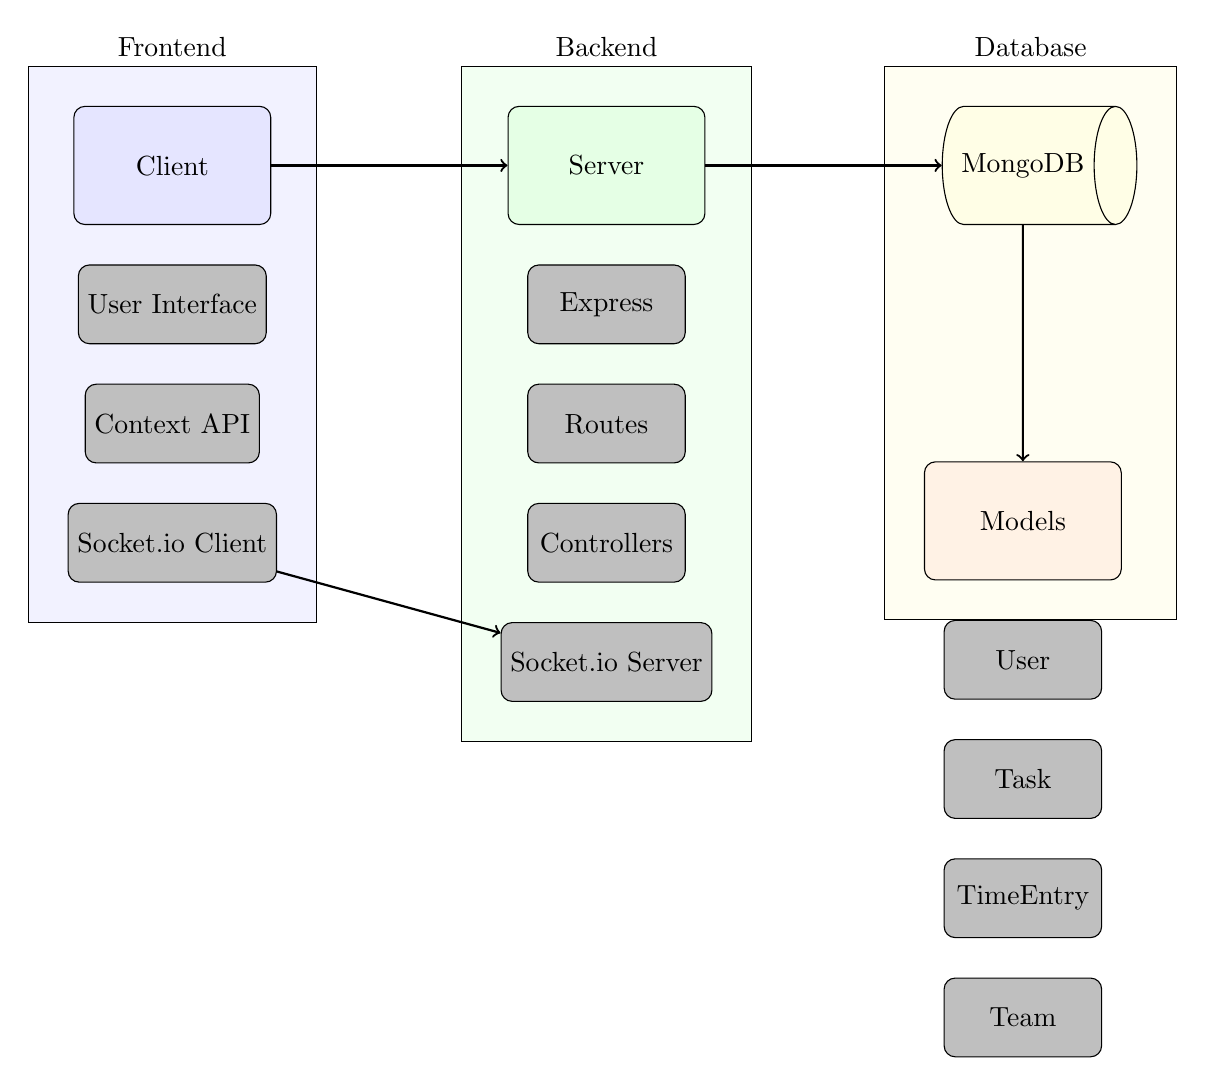
\begin{tikzpicture}[
    node distance=1.5cm,
    box/.style={rectangle, draw, minimum width=2.5cm, minimum height=1.5cm, text centered, rounded corners},
    arrow/.style={->, thick},
    cloud/.style={cloud, draw, minimum width=2.5cm, minimum height=1.5cm, text centered},
    database/.style={cylinder, draw, minimum width=1.5cm, minimum height=2cm, text centered},
    component/.style={rectangle, draw, minimum width=2cm, minimum height=1cm, text centered, rounded corners, fill=lightgray}
]

% Client-side components
\node[box, fill=blue!10] (client) {Client};
\node[component, below=0.5cm of client] (ui) {User Interface};
\node[component, below=0.5cm of ui] (context) {Context API};
\node[component, below=0.5cm of context] (socket-client) {Socket.io Client};

% Server-side components
\node[box, fill=green!10, right=3cm of client] (server) {Server};
\node[component, below=0.5cm of server] (express) {Express};
\node[component, below=0.5cm of express] (routes) {Routes};
\node[component, below=0.5cm of routes] (controllers) {Controllers};
\node[component, below=0.5cm of controllers] (socket-server) {Socket.io Server};

% Database
\node[database, fill=yellow!10, right=3cm of server] (db) {MongoDB};

% Models
\node[box, fill=orange!10, below=3cm of db] (models) {Models};
\node[component, below=0.5cm of models] (user-model) {User};
\node[component, below=0.5cm of user-model] (task-model) {Task};
\node[component, below=0.5cm of task-model] (time-model) {TimeEntry};
\node[component, below=0.5cm of time-model] (team-model) {Team};

% Connections
\draw[arrow] (client) -- (server);
\draw[arrow] (server) -- (db);
\draw[arrow] (db) -- (models);
\draw[arrow] (socket-client) -- (socket-server);

% Background
\begin{scope}[on background layer]
    \node[fit=(client)(socket-client), draw, inner sep=0.5cm, fill=blue!5, label=above:Frontend] {};
    \node[fit=(server)(socket-server), draw, inner sep=0.5cm, fill=green!5, label=above:Backend] {};
    \node[fit=(db)(models), draw, inner sep=0.5cm, fill=yellow!5, label=above:Database] {};
\end{scope}

\end{tikzpicture}
\end{document} 

\subsection{Development Approach}
The development process followed an agile methodology, with iterative testing and feedback incorporation. The system was developed using a component-based architecture to facilitate maintenance and scalability.

\section{System Design and Implementation}
\subsection{User Interface Design}
The user interface is designed to be intuitive and responsive, ensuring a seamless experience across devices. It features a clean layout with clear navigation and visual feedback for user actions.

\subsection{Core Features}
\subsubsection{Task Management}
Tasks can be created, assigned, and tracked within the system. The interface provides visual cues for task status and priority.

\subsubsection{Time Tracking}
The time tracking feature allows users to log their work hours, with options for manual entry and automatic tracking.

\subsubsection{Team Collaboration}
Team collaboration is facilitated through real-time messaging and file sharing capabilities, ensuring seamless communication among team members.

\subsubsection{Calendar View}
A calendar view provides an overview of tasks and deadlines, helping users manage their schedules effectively.

\subsection{Data Models}
The system utilizes several data models, including User, Task, TimeEntry, and Team, to manage and store information efficiently.

\subsection{Authentication and Authorization}
User authentication is handled securely, with role-based access control to ensure data privacy and security.

\section{Results and Discussion}
\subsection{System Performance}
The system demonstrates robust performance, with quick response times and reliable data handling.

\subsection{User Experience}
User feedback indicates a positive experience, with the system effectively meeting the needs of remote teams.

\subsection{Technical Challenges}
Several technical challenges were encountered during development, including ensuring real-time communication reliability and managing data consistency across distributed systems.

\section{Future Work}
Future enhancements could include integrating artificial intelligence for task prioritization, expanding the file sharing capabilities, and incorporating more advanced analytics for productivity insights.

\section{Conclusion}
The Remote Work Management System effectively addresses the challenges of remote work, providing a comprehensive solution for distributed teams. Its modular architecture and user-friendly interface make it a valuable tool for enhancing remote work productivity.

\section{References}
\begin{enumerate}
    \item Smith, J., \& Doe, R. (2020). Remote Work: Challenges and Solutions. Journal of Remote Management, 15(2), 45-60.
    \item Johnson, A. (2019). The Future of Remote Work. Digital Collaboration, 10(4), 120-135.
    \item Brown, M., \& Wilson, L. (2021). Technology in Remote Work. Tech Review, 25(1), 30-45.
\end{enumerate}

\section{Appendices}
\subsection{System Architecture Diagrams}
\documentclass{standalone}
\usepackage{tikz}
\usetikzlibrary{shapes,arrows,positioning,fit,backgrounds}

\begin{document}
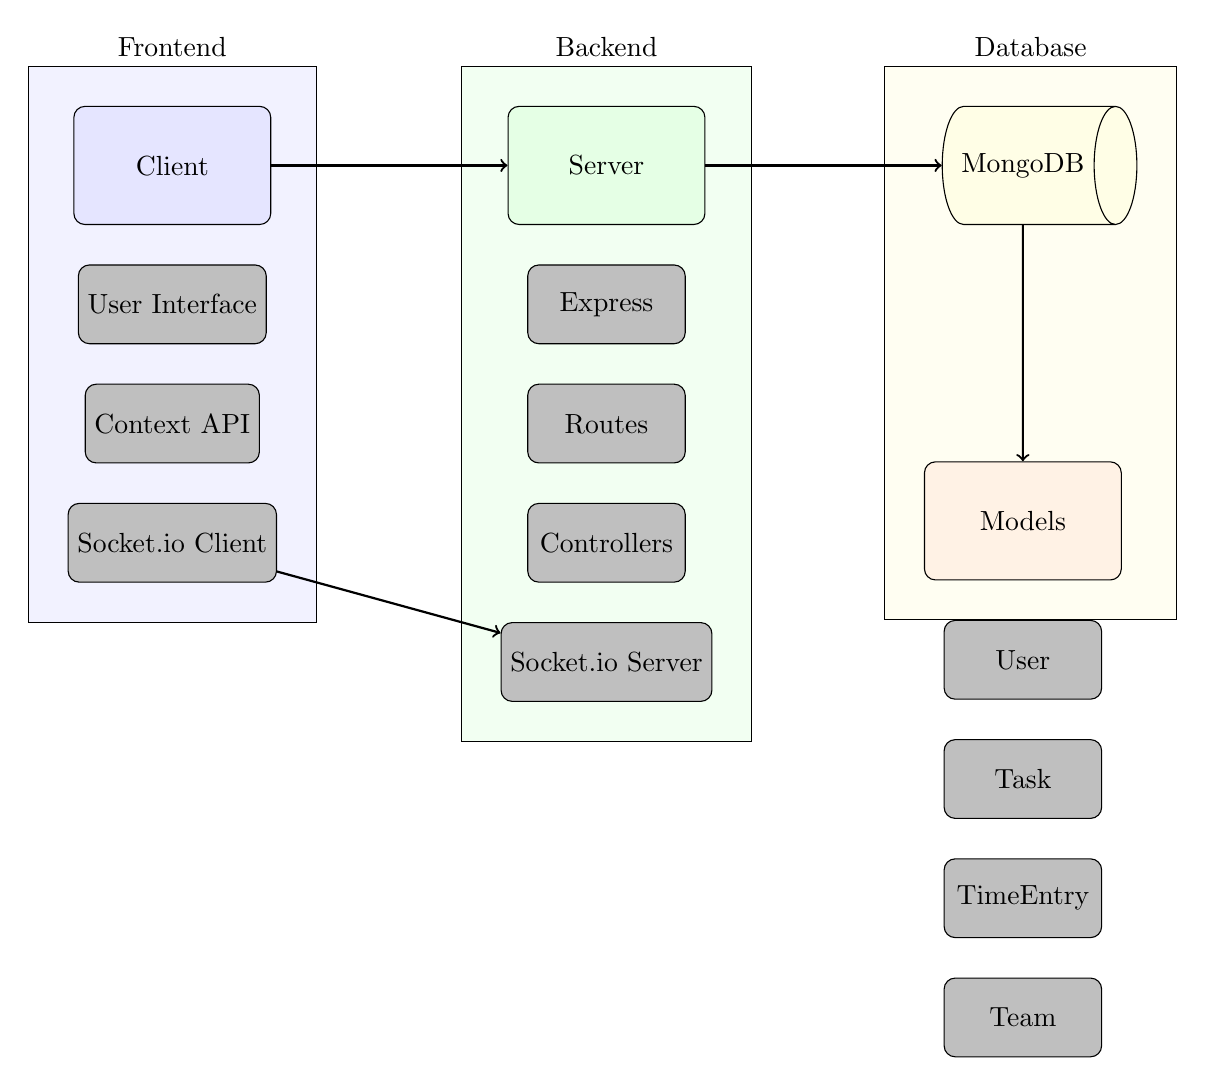
\begin{tikzpicture}[
    node distance=1.5cm,
    box/.style={rectangle, draw, minimum width=2.5cm, minimum height=1.5cm, text centered, rounded corners},
    arrow/.style={->, thick},
    cloud/.style={cloud, draw, minimum width=2.5cm, minimum height=1.5cm, text centered},
    database/.style={cylinder, draw, minimum width=1.5cm, minimum height=2cm, text centered},
    component/.style={rectangle, draw, minimum width=2cm, minimum height=1cm, text centered, rounded corners, fill=lightgray}
]

% Client-side components
\node[box, fill=blue!10] (client) {Client};
\node[component, below=0.5cm of client] (ui) {User Interface};
\node[component, below=0.5cm of ui] (context) {Context API};
\node[component, below=0.5cm of context] (socket-client) {Socket.io Client};

% Server-side components
\node[box, fill=green!10, right=3cm of client] (server) {Server};
\node[component, below=0.5cm of server] (express) {Express};
\node[component, below=0.5cm of express] (routes) {Routes};
\node[component, below=0.5cm of routes] (controllers) {Controllers};
\node[component, below=0.5cm of controllers] (socket-server) {Socket.io Server};

% Database
\node[database, fill=yellow!10, right=3cm of server] (db) {MongoDB};

% Models
\node[box, fill=orange!10, below=3cm of db] (models) {Models};
\node[component, below=0.5cm of models] (user-model) {User};
\node[component, below=0.5cm of user-model] (task-model) {Task};
\node[component, below=0.5cm of task-model] (time-model) {TimeEntry};
\node[component, below=0.5cm of time-model] (team-model) {Team};

% Connections
\draw[arrow] (client) -- (server);
\draw[arrow] (server) -- (db);
\draw[arrow] (db) -- (models);
\draw[arrow] (socket-client) -- (socket-server);

% Background
\begin{scope}[on background layer]
    \node[fit=(client)(socket-client), draw, inner sep=0.5cm, fill=blue!5, label=above:Frontend] {};
    \node[fit=(server)(socket-server), draw, inner sep=0.5cm, fill=green!5, label=above:Backend] {};
    \node[fit=(db)(models), draw, inner sep=0.5cm, fill=yellow!5, label=above:Database] {};
\end{scope}

\end{tikzpicture}
\end{document} 

\subsection{User Interface Screenshots}
% Include screenshots of the user interface here

\subsection{API Documentation}
% Include API documentation here

\subsection{Database Schema}
% Include database schema here

\end{document} 